\documentclass[twoside]{article}
\usepackage[left=3cm, right=3cm, top=0cm]{geometry}
\usepackage{amsmath}
\usepackage{mathtools}
\usepackage{tikz}
\usepackage{hyperref}
\hypersetup{
    colorlinks,
    citecolor=green,
    filecolor=black,
    linkcolor=blue,
    urlcolor=blue
}
\usepackage{tikz,fullpage}
\usetikzlibrary{arrows,%
                petri,%
                topaths}%
\usepackage{tkz-berge}
\usepackage[position=top]{subfig}
\usetikzlibrary{arrows,%
                petri,%
                topaths}%
\setlength{\parindent}{0pt}
\begin{document}

\title{Project on Optimization}
\author{Jacob Puthipiroj}
\date{}
\maketitle

\section*{Introduction}
The sports industry is huge. Even within a one league of one single sport, revenues can amount to over billions of dollars per season. The investment of capital in creating a marketable sports tournament is similarly enormous: the booking of stadiums and television slots, the salaries of coaches and players, the pre-game advertising and post-game roundup. Executives have every incentive to maximize the profits of each game while adhering to constraints imposed by the industry. Consequently, the once mundane scheduling of games $-$ the specification of when, where, and which teams play each other $-$ becomes a mathematical optimization problem capable of saving millions of dollars. \\

In this paper, I explore a constraint-programming approach to this optimization problem in the context of a scheduling a Major League Soccer tournament. The setup is as follows: \\

 \textbf{Objective Function}: The total distance traveled altogether by teams, to be minimized. \\
  \textbf{Decision Variables}: The trip start dates for each team. \\ 
 \textbf{Constraints}: Each team cannot play more than two consecutive games away from home. Each team must play all other teams exactly once. \\

As shown in the \href{https://docs.google.com/spreadsheets/d/1eGgyUOwjtrGtbim5T5FRE0Uae482cQo0NV0-RXekXss/edit?usp=sharing}{final spreadsheet}, this implementation led to the saving of over 10,000 kilometers of travel for a 5-team problem. When scaled up to real situations, this could result in saving millions in transportation and accommodation costs, as well as latently boosting revenues by allowing better performance from well-rested athletes.

\section*{Model Uncertainty and Sensitivity Analysis}


Unlike blending problems, where the certainty assumption of certain parameters are dubious and sensitivity analysis is helpful in understanding the stability of optimal solutions, tournament scheduling problems have relatively fixed parameters. It is incoherent, say, to alter the distance matrix in theory, as cities cannot move in practice. Interestingly, Kostuk (2012) broadens the definition of sensitivity analysis in the TPP as `how does the optimal schedule distance change given different schedule constraints'? \\

The paper explicitly mentions an `iterative process arriving a definitive schedule', whereby three or four different bounce back and forth between them as the details are fine-tuned to incorporate new constraints\footnote{\#modelSensitivityandUncertainty: I address the problem of performing useful sensitivity analysis in fixed-parameter problems and provide a workaround by broadening the definition of sensitivity analysis, while citing the relevant literature.}. Some of these constraints were based on team popularity, e.g. the four teams with the lowest drawing power should not play each other in the first 5 rounds because attendance would be low, while each of the three most popular teams must play exactly one classic matchup at home. The authors did not report optimal solution distances given any, or even all of these constraints, but instead reported that the value of the feasible solution in the objective function was 5.6\% better than in the relaxed problem. Surprisingly, constraining the problem lead to an \textit{improvement}, rather than a reduction in quality of the solution. This was partially due to the nature of the objective function itself; instead of the total distance traveled by all teams, a unit of distance to be minimized (as in the implementation), the authors aimed to maximize the `concentration of games between teams within the same group towards the final round of the tournament'.

\section*{Implementation Challenges }
This was a difficult problem; deliberately so in order to simulate a real-world problem that would be impossible to solve by hand. There were many problems encountered:
\begin{enumerate}
\item \textbf{Understanding the correct approach:} Instead of considering one game at a time (between two teams), I intuited that each team would have its own optimal (minimum) schedule, and hopefully the total optimal schedule will contain all optimal sub-schedules.
\item \textbf{Constructing the single-team solution:} This is itself a linear optimization problem, with the most difficult part being the constraint against two-cycles. The was resolved by creating a variable for the total number of trips going in and out of each city pair, limited to 1 at most.
\item \textbf{Combining the single-team solutions}: A major breakthrough came when realizing that reverse trips were fundamentally different from forward trips, and helped to break the symmetry of the solution. Instead of 2 trips $\times$ 10 days  = 20  decision variables, using 4 trips (2 forward, 2 reverse) $\times$ 10 days allowed easy and accurate encoding of certain difficult constraints, including the ``no 3 consecutive home/away games" rule.\footnote{\#breakitdown: I effectively decompose a problem into tractable, clear, and well defined components (the whole schedule into simply the schedule for each individual city); accurately combines component solutions into a full solution (by finding linear combinations of each of the 5 subtours on different days).}

\end{enumerate}


\section*{Generalizable Lessons}
\subsection*{Obtain Optimal Patterns by combining Optimal Subpatterns}

Constraint Programming can accompany Integer Programming in order to make it much more powerful. The article specifically mentions this in terms of feasible `patterns' obtained from each team which were either explicitly or implicitly assigned. This was directly used in the implementation. The optimal tour for Denver, for example, is as follows:\\
\begin{figure}[h!]

\begin{center} 
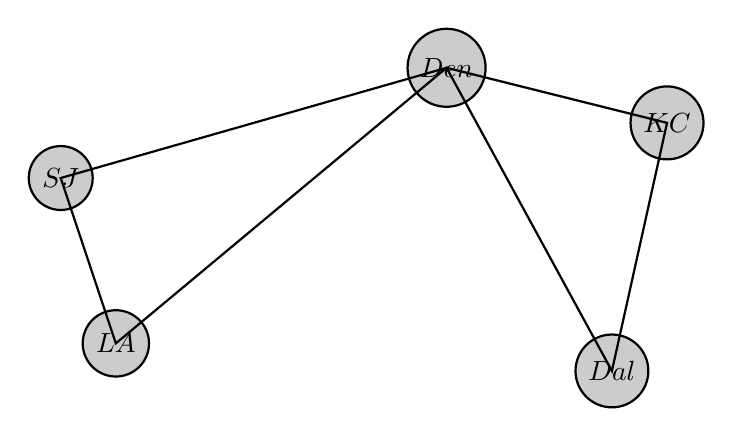
\begin{tikzpicture}[scale=.7,colorstyle/.style={circle, draw=black!100,fill=black!20, thick, inner sep= 3pt, minimum size=3mm}]
    \node (n1) at (0,0)[colorstyle]{$LA$};
    \node (n2) at (-1,3)[colorstyle]{$SJ$};
    \node (n3) at (6,5)[colorstyle]{$Den$};
    \node (n4) at (10,4)[colorstyle]{$KC$};
    \node (n5) at (9,-0.5)[colorstyle]{$Dal$};
    \draw[thick](6,5)--(-1,3)--(0,0)--(6,5)--(9,-0.5)--(10,4)--(6,5);
\end{tikzpicture}
\end{center} 
\end{figure}

The pattern is clear: make one trip to the two closest cities, and another to the two furthest cities\footnote{\#dataviz: This visualization creates new, significant insights into the construction of optimal subtours for each team.}. By hardcoding this pattern into the solution, it is easy to see that, say, for KC, its optimal tour will be one of (Den-Dal or Dal-Den) $\times$(SJ-KC or KC-SJ) = 4 total paths. The final schedule are thus linear combinations of $4\times5=20$ different paths - clearly, a computationally tractable number.\footnote{\#entObjectivesandConstraints: The constraint that that each team cannot play more than two consecutive games away from home would normally be a soft constraint (should be obeyed), rather than a hard one (must be obeyed). However, by making it a hard constraint, and turning the problem into a constraint programming one, I find an optimal feasible solution for the soft constraint instance.}\footnote{\#constraints: Actually, not only did I find a solution that respects the constraints, I would not have been able to find an optimal solution (at least in Sheets) without it. This constraint was a blessing, because it significantly reduced the search space from $20!/2^{10} \approx 10^{15}$ to about $10^{5}$.}

\section*{Insights Regarding LOs}
The TPP is a `notoriously difficult problem', but educationally rewarding. Not only did I successfully minimize the objective function - the schedule distance -  to within 4.6\% of the theoretical minimum, but did so within the context of realistic constraints - that teams may not spend more than 2 consecutive games away from home. In fact, this problem was only solveable in Excel \textit{because} the constraints allowed the search space to be reduced via constraint programming.\\ 

This assignment also provided an interesting take on the concept of \#modelSensitivityandUncertainty by broadening the definition of `Sensitivity Analysis' to include fixed-parameter/roughly deterministic problems. In fact, the nature of the problem revealed how closely the two LOs interact, since the primary method for reducing model sensitivity to the uncertainties of the real world was through the addition of model constraints!




\newpage
\twocolumn

\section*{Implementation Appendix}
\subsection*{1 The Single Team Problem}

\subsubsection*{Decision Variables}

The games are defined using $\forall i \neq j \in I$ (the set of teams) as the following binary variables:
$$ x_{ij} = 
\begin{cases} 
	1 & \textrm{if team $i$ plays against home team $j$} \\
	0 & \textrm{otherwise} \\
\end{cases}$$
\subsubsection*{Variables}
$$ d_{ij} = \textrm{the distance between city $i$ and home team $j$} $$
\subsubsection*{Objective Function}

For a single team $i$, the objective is the total distance for it to travel to all the cities 

$$\sum_{i=1}^5 \sum_{i=1}^5 d_{ij}x_{ij}, \quad x_{ii} =0 $$
In practice, $d_{ii}$ was made large enough that $x_{ii}$ was never chosen, effectively making $x_{ii} = 0$.
\subsubsection*{Constraint Function}
Team $i$ must enter all other cities eactly once and leave all other cities exactly once.
$$\sum_{j \neq i} x_{ij} = 1 \textrm{ for all } i \neq1$$ $$  \sum_{i \neq j} x_{ij} = 1 \textrm{ for all } j \neq 1  $$
However, team $i$ will exit its city exactly twice, and return to its city exactly twice.
$$\sum_{j \neq i} x_{ij} = 2 \textrm{ for } i  =1 $$ $$  \sum_{i \neq j} x_{ij} = 1 \textrm{ for } j = 1  $$
In order to avoid 2-cycles, each pair of cities $i$ and $j$ can have at most one enter or exit status.
$$ x_{ij} + x_{ji} \leq 1$$

\newpage
\
\subsection*{2 The Multiple Team Problem}
\subsubsection*{Decision Variables}
In this problem, there is a distinct difference between going on a tour, and going on it in reverse. $i.e, \ (a \to b\to c\to a ) \neq (a \to c \to b\to a)$
$$ y_{ijk} = 
\begin{cases} 
	1 & \textrm{if team $i$ starts trip $j$ on day $k$} \\
	0 & \textrm{otherwise} \\
\end{cases}$$
$$ z_{ijk} = 
\begin{cases} 
	1 & \textrm{if team $i$ starts trip $j$ in reverse on day $k$} \\
	0 & \textrm{otherwise} \\
\end{cases}$$
\subsubsection*{Variables}
$$ d_{ij} = \textrm{the distance between city $i$ and home team $j$} $$
\subsubsection*{Objective Function}
For all teams, the objective is the total distance traveled to all cities.
$$ \sum_{j=1}^{5}\sum_{i=1}^{5}\sum_{k=1}^{10}d_{ij}y_{ijk} + \sum_{j=1}^{5}\sum_{i=1}^5\sum_{k=1}^{10} d_{ij}z_{ijk} $$
\subsubsection*{Constraint Functions}
Exactly one forward/reverse trip is allowed per $j$. 
$$ \sum_{k=1}^{10}y_{ijk} + \sum_{k=1}^{10}z_{ijk} \leq 1 \textrm{ for all $i = 1 , ... , 5, j = 1,2$}$$
Teams may not have two road trips in a row.
$$ \sum_{k=l}^{\mathclap{l + 2 \textrm{ mod}  \ 10}} (y_{i1k} + y_{i2k} + z_{i1k} + z_{i2k} ) \leq 1 \textrm{ for $l = 1,...,10$}$$
Home teams must be present when visitors arrive.
\begin{align*}
\sum_{\mathclap{l \neq i, i \textrm{ first in }j(i,l)}} &(y_{lj(i,l)k} + z_{lj(i,l)(k-1)\textrm{mod}10}) \quad + \\
\sum_{\mathclap{l \neq i, i \textrm{ second in }j(i,l)}} &(y_{lj(i,l)(k-1)\textrm{mod}10} \ + z_{lj(i,l)k}) 
\end{align*}
$$\leq 1 - \sum_{{m=(k-1)\textrm{mod}10}} \sum_{j=1,2}(y_{ijm} + z_{ijm}) $$
$$\textrm{ for $k = 1, ..., 10; i = 1,...,5$}$$\footnote{\#optimization: For the whole appendix, as well as the google Sheets implementation.}

\newpage
\newgeometry{left=3cm,right = 3cm,bottom=0.1cm}
\onecolumn

\bibliographystyle{plain}
\nocite{*}
\bibliography{bibfile.bib}

\end{document}